%-------------------------
%clang
%(c) H.Buchmann FHNW 2008
%export TEXINPUTS=.:${HOME}/fhnw/edu/:${HOME}/fhnw/edu/tinL/config/latex:${HOME}/fhnw/edu/config//:
%-------------------------
\documentclass{beamer}
\usepackage{beamer}
%---------------------
%local defines
%(c) H.Buchmann FHNW 2009
%$Id$
%---------------------
\newcommand{\target} {\beaglebone\xspace}
\newcommand{\targetS}{{\bf BBG}\xspace}
\newcommand{\host}   {{\em Host}\xspace}
\newcommand{\targetroot} {{\bf target-root}\xspace}
\newcommand{\kernel} {{\bf kernel}\xspace}
\renewcommand{\c}{{\bf C}\xspace}
\newcommand{\cpp}{{\bf C++}\xspace}
\newcommand{\posix}{{\bf POSIX}\xspace}

\input{/home/buchmann/latex/dirtree/dirtree.tex}
\newcommand{\kernelmodule}{{\em kernelmodule}\xspace}
\renewcommand{\src}[1]{#1}

\usepackage[absolute]{textpos}
\setlength{\TPHorizModule}{1mm}
\setlength{\TPVertModule}{1mm}

\begin{document}
\begin{frame}{Um was geht es ?}
 \begin{itemize}
  \item \linux \kernelmodule's
  \begin{itemize}
   \item userspace
   \item kernelspace: wo die \kernelmodule sind
  \end{itemize}
  \item Herstellung
  \item Interrupts
 \end{itemize}
\end{frame}

\begin{frame}{Userspace-Kernelspace}{zwei verschiedene Welten}
 \begin{center}
 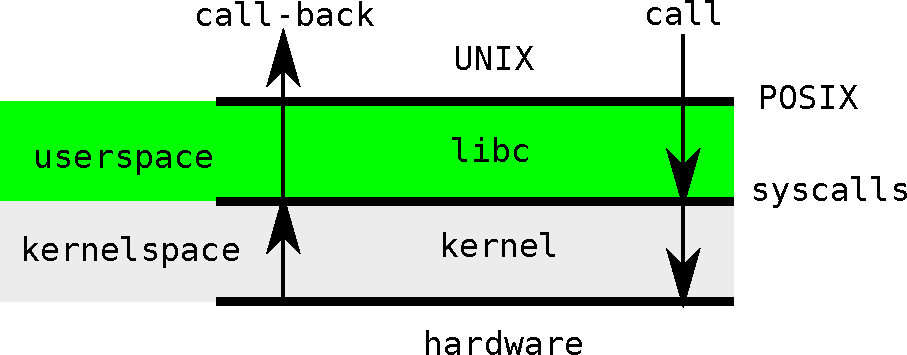
\includegraphics[width=0.75\textwidth]{userspace-kernelspace.pdf}
 \end{center}
\end{frame}

\begin{frame}{\cod{syscall.c}}{Beispiel userspace}
 \begin{itemize}
  \item \cod{syscall}
  \item der File \cod{sys/syscall.h}
 \end{itemize}
\end{frame}

\begin{frame}{Verzeichnisstruktur}{auf dem \host}
\dirtree{%
 .1 17-build.
 .2 modules \DTcomment{source and generated files}.
 .3 Makefile \DTcomment{for the modules}.
 .2 scripts.
 .3 modules.sh \DTcomment{wrapper to make}.
}
\end{frame}

\begin{frame}{Der Workflow}{die Orte}
 \vspace{-2mm}
 \begin{description}[\target]
  \item[\host] \cod{17-build/modules}
  \item[\target]\cod{/work}
  \item[Verbindung] mit \cod{scp} (secure copy)
   \begin{description}
   \item[Server] \cod{sshd} \target
   \item[Client] \host
  \end{description}
 \end{description}
\end{frame}

\begin{frame}{Der Workflow}
 \begin{tabular}{c|p{6.5cm}|p{3.5cm}}
   & \host						& \target\\
   \hline
  A&Edititiere \cod{\em a-module.c} 			&	\\
  B&\cod{sh scripts/module.sh {\em a-module.ko}}	&	\\
  C&\cod{scp a-module.ko roo@ip:/work} 			&	\\
  D&							& \cod{insmod {\em a-module.ko}}\\
  E&							& teste\\
  F&							& \cod{rmmod {\em a-module.ko}}\\
\hline
   & $\to$A\\
 \end{tabular}
\end{frame}

\begin{frame}{Die Schritte}
 \begin{description}[\src{simple-ioctl.c|h}]
  \item[\src{simple-module.c}]\hfill
  \vspace{-5mm}
  \begin{itemize}
   \item \cod{insmod}/\cod{rmmod}
   \item debug mit \cod{printk}
  \end{itemize}
  \item[\src{simple-device.c}]\hfill
  \vspace{-5mm}
  \begin{itemize}
   \item das Konzept {\em File}: alles ist ein File
   \item \cod{read}, \cod{write} \& Co.
  \end{itemize}
  \item[\src{simple-ioctl.c|h}] \hfill
  \vspace{-5mm}
  \begin{itemize}
   \item Einstellungen mit \cod{ioctl}
  \end{itemize}
  \item[\src{simple-hw.c}] \hfill
  \vspace{-5mm}
  \begin{itemize}
   \item Zugriff auf die Hardware
  \end{itemize}
  \item[\src{simple-irq.c}]\hfill
  \vspace{-5mm}
  \begin{itemize}
   \item interrupts
   \begin{itemize}
    \item {\em foreground} der {\em handler}
    \item {\em background} 
    \item {\em tasklet} die Verbindung {\em foreground}$\to${\em background} 
   \end{itemize}
  \end{itemize}
 \end{description}
\end{frame}


\begin{frame}{Ziel}{\cod{simple-module.c}}
 \begin{itemize}
  \item Herstellung 
  \item install/deinstall
  \item elementare call-backs
 \end{itemize}
\end{frame}

\begin{frame}[fragile]{\src{simple-module.c}}{init/exit}
 \begin{lstlisting}
module_init(simple_init); /* register  :called by kernel */
module_exit(simple_exit); /* deregister:called by kernel */
 \end{lstlisting}
 \begin{itemize}
  \item call-back
  \item register/deregister
  \item \cod{printk} wie \cod{printf}
  \begin{lstlisting}
    printk(KERN_INFO "%d %x",val1,val2);
  \end{lstlisting}
  für debug
 \end{itemize}
\end{frame}

\subsection{Aufgaben}
\begin{frame}{Aufgaben}
 \begin{itemize}
  \item \url{src/simple-module.c} für \host/\targetS
  \item Machen Sie eine 'ewige Schlaufe'
  \end{itemize}
\end{frame}


\begin{frame}{Ziel}{\src{simple-device.c}}
 \begin{itemize}
  \item Verbindung {\em userspace}-{\em userspace}
  \begin{itemize}
   \item alles ist ein File
  \end{itemize}
  \item {\em devicefile} 
  \begin{itemize}
   \item \cod{mknod {\em device-file} {\em type} major minor}
  \end{itemize}
  \item die elementaren Operationen
 \end{itemize}
\end{frame}

\subsection{userspace: alles ist ein File}
\begin{frame}{\src{simple-device.c}:im alles ist ein File}
             {Die elementaren Operationen im {\em userspace}}
 \vspace{-4mm}
  \begin{itemize}
   \item \cod{open}
   \item \cod{read}
   \item \cod{write}
   \item \cod{close}
  \end{itemize}
\end{frame}

\begin{frame}{Die elementaren Operationen im {\em userspace}}
             {der Befehl \cod{cat}}
  \begin{itemize}
   \item \cod{cat {\bf device}}
   \begin{itemize}
    \item \cod{open},\cod{read},\cod{close}
   \end{itemize}
   \item \cod{cat file > {\bf device}}
   \begin{itemize}
    \item \cod{open},\cod{write},\cod{close}
   \end{itemize}
  \end{itemize}
\end{frame}

\begin{frame}{Der Devicefile \cod{device}}
 \begin{itemize}
  \item ist ein File
  \item bezeichnet ein {\em device}
  \item ist normalerweise im Verzeichnis \cod{dev}
  \begin{itemize}
   \item muss aber nicht 
  \end{itemize}
 \end{itemize}
 \begin{block}{Beispiele}
  \begin{itemize}
   \item \cod{/dev/ttyUSB0} die serielle Schnittstelle
   \item \cod{/dev/mmcblk0} die SD-Karte auf \target
   \item \cod{/dev/random}, \cod{/dev/urandom}
   \item ...
  \end{itemize}
 \end{block}
\end{frame}

%\begin{frame}{Beispiele}{alles ist ein File}
%{\cod{/dev/random}, 
%\cod{/dev/urandom}, \cod{/dev/sda}}
% \begin{itemize}
%  \item \cod{cat /dev/random | hexdump -C} 
%  \begin{itemize}
%    \item sammelt das Rauschen: langsam
%   \end{itemize}
%  \item \cod{dd if=/dev/sda count=1 | hexdump -C}
%  \begin{itemize} 
%    \item der MBR 
%  \end{itemize}  
% \end{itemize}
%\end{frame}

\begin{frame}[fragile]{Die Verbindung {\em file - device}}{Devicefile}
\begin{block}{Beispiel: \cod{/dev/ttyUSB0}\footnote{gemacht mit \cod{ls -l}}}
\vspace{-5mm}
{\footnotesize
\begin{verbatim}
crw-rw---- 1 root uucp   188,  0 11. Nov  20:27 /dev/ttyUSB0
|            |    |      |     |                |
|            |    |      |     |                name
|            |    |      |     minor                
|            |    |      major 
|            |    group 
|            owner
devicetyoe
\end{verbatim}
}
\end{block}
\vspace{-6mm}
\begin{block}{f�r uns wichtig:}
 \vspace{-3mm}
 \begin{description}
  \item[major] Code f�r die {\em device} Klasse
  \item[minor] Nummer f�r ein {\em device} 
 \end{description}
\end{block}
\end{frame}

\begin{frame}{Major:Minor}{objektorientierte Interpretation}
 \begin{description}
  \item[major] Code f�r die {\Large Klasse}
  \item[major] Code f�r die {\Large Instanz}
 \end{description}
\end{frame}

\begin{frame}[fragile]{Der Befehl \cod{mknod}}{erzeugt einen {\em Devicefile}}
\begin{verbatim}
Usage: mknod [-m MODE] NAME TYPE MAJOR MINOR                                    
                                                                                
Create a special file (block, character, or pipe)                               
                                                                                
        -m MODE Creation mode (default a=rw)                                    
TYPE:                                                                           
        b       Block device                                                    
        c or u  Character device                                                
        p       Named pipe (MAJOR and MINOR are ignored)                        
\end{verbatim} 
\end{frame}

\subsection{kernelspace}
\begin{frame}[fragile]{\cod{register\_chrdev}}
 \begin{itemize}
  \item erzeugt {\em major}
  \item \cod{file\_operations fops} die Fileoperationen
  \begin{itemize}
   \item call-backs
   \item siehe \cod{linux/fs.h}
  \end{itemize}
 \end{itemize}
 \begin{block}{� la \CPP}
 \begin{lstlisting}
  class File
  {
   protected:
    virtual int open(...)=0;
    virtual int flush(...)=0;
    virtual int read(...)=0;
    virtual int write(...)=0;
    ...
  };
 \end{lstlisting}
 \end{block}
 
\end{frame}

\begin{frame}{Transfer userspace $\leftrightarrow$ kernelspace}
{\cod{simple-read} und \cod{simple-write}}
\begin{center}
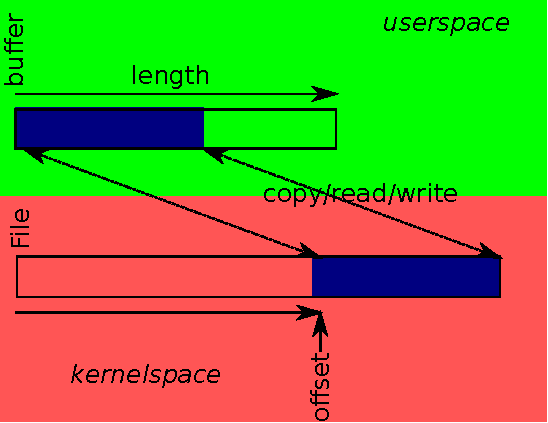
\includegraphics[height=0.75\textheight]{user-kernel-space-copy.pdf}
\end{center}
\end{frame}


\subsection{Test}
\begin{frame}{Test}
 \begin{itemize}
  \item \cod{insmod simple-device.ko}
  \begin{itemize}
   \item $\to major$
  \end{itemize}
  \item \cod{mknod devi c {\em major} {\em i}}
  \begin{itemize}
   \item Devicefile beliebige minor
  \end{itemize}
  \item \cod{cat devi}
  \begin{itemize}
   \item lese von \cod{devi}
  \end{itemize}
  \item \cod{echo "{}hello"{} > devi}
  \begin{itemize}
   \item schreibe auf \cod{devi}
  \end{itemize}
 \end{itemize}
 \remark{\cod{devi} in \cod{/work}}
\end{frame}

\subsection{Aufgaben}
\begin{frame}{Aufgaben}
\begin{itemize}
 \item \cod{src/simple-device.c} f�r \host/\targetS
 \item Registrierung/Deregistrierung  in \cod{sys/class}
 \begin{itemize}
  \item  \cod{class\_create}
  \item  \cod{device\_create}
 \end{itemize}
\end{itemize}
\end{frame}


%\begin{frame}{simple-device}{userspace$\leftrightarrow$kernelspace}
% \begin{itemize}
%  \item alles ist ein File
%  \begin{itemize}
%   \item {\em stream of bits}
%  \end{itemize}
%  \item Trennung {\bf userspace} {\bf kernelspace}
%  \begin{itemize}
%   \item meltdown, spectre
%  \end{itemize}
% \end{itemize}
%\end{frame}
%
%\begin{frame}{simple-device}
% \begin{description}
%  \item[Module] \cod{src/simple-device.c}, \cod{src/Makefile}
%  \item[Test] 
%     \begin{itemize}
%       \item \cod{insmod simple-device.ko} Major Number
%       \item \cod{mknod -ma=rw simple c Major 1} Device File Zugriff f�r alle
%       \item \cod{cat simple} read 
%       \item \cod{cat aFile > simple} write
%     \end{itemize} 
% \end{description}
% \begin{todos}
%  \item Automatische Erzeugung von \cod{simple}
%  \item die \cod{file\_operations}: \cod{open} und \cod{close}
% \end{todos}
%\end{frame}
%
%\begin{frame}{\cod{simple-device.c}}{userspace $\leftrightarrow$ kernelspace}
% \begin{description}[kernelspace $\to$ userspace]
%  \item[Module] brauche  \cod{print\_hex\_dump} eine praktische Funktion
%  \item[userspace $\to$ kernelspace] \cod{simple\_write}
%  \item[kernelspace $\to$ userspace] \cod{simple\_read}
%  \item[Test] \cod{simple-device} im userspace
% \end{description}
% \todo{Erzeuge Absturz}
%\end{frame}

\begin{frame}{Problem}
\begin{itemize}
 \item Funktioniert f�r \host
 \item Funktioniert {\Huge nicht} f�r \targetS
\end{itemize}
\end{frame}

\begin{frame}{Ziel}{\src{simple-ioctl.c|h} und \src{simple-ioctl-userspace.c}}
 \begin{itemize}
  \item Einstellungen
  \item \cod{ioctl(fileId,cmd,data)}
 \end{itemize}
\end{frame}

\begin{frame}{ioctl - control device}{userspace}
\begin{itemize}
 \item \cod{man 2 ioctl}
\begin{quote}
{\footnotesize
The  {\bf ioctl()} function manipulates the underlying device parameters of special
files.  In particular, many operating characteristics of character special files
(e.g., terminals) may be controlled with {\bf ioctl()} requests.  The argument d
must be an open file descriptor
}
\end{quote}
 \item \cod{int ioctl(int d, unsigned long request, ...);}
\end{itemize}
\end{frame}

\begin{frame}[fragile]{Im userspace}{\src{simple-ioctl-userspace.c}}
\begin{itemize}
 \item die {\em requests} \src{simple-ioctl.h}
 \begin{lstlisting}
#define SIMPLE_IOCTL_WRITE _IOW(0x23,5,int)  
#define SIMPLE_IOCTL_READ  _IOR(0x23,5,int) 
 \end{lstlisting}
 \item \src{simple-ioctl-userspace.c}
 \begin{itemize}
  \item read
  \vspace{-2mm}
  \begin{lstlisting}
int val=1;
int res=ioctl(id,SIMPLE_IOCTL_READ,&val);
  \end{lstlisting}
  \item write
  \vspace{-2mm}
  \begin{lstlisting}
int res=ioctl(id,SIMPLE_IOCTL_WRITE,0x1234);
  \end{lstlisting}
 \end{itemize}
\end{itemize}
\end{frame}

\begin{frame}{Test}{siehe \src{simple-device.c} Test}
 \begin{itemize}
  \item \cod{insmod}
  \item \cod{mknod}
  \item \cod{./simple-ioctl-userspace}
 \end{itemize}
\end{frame}

\section{\src{simple-hw.c}}
\begin{frame}{Ziel}{\src{simple-hw.c}}
 \begin{itemize}
  \item iomem
  \begin{itemize}
   \item  mapping
  \end{itemize}
 \end{itemize}
\end{frame}

\begin{frame}[fragile]{ioremap/iounmap}
\begin{itemize}
 \item der \cod{struct} FPGA
 \item iomem
\begin{lstlisting}
 fpga=(FPGA* __iomem)ioremap(FPGA_BASE,FPGA_SIZE); 
                     /* reserve memory */
 iounmap(fpga);
\end{lstlisting}
\end{itemize}
\end{frame}

\begin{frame}{Test}{siehe \src{simple-device.c} Test}
 \begin{itemize}
  \item \cod{insmod}
  \item \cod{mknod}
  \item read: \cod{cat {\em device}}
  \item write:\cod{cat {\em file} > {\em device}}
 \end{itemize}
\end{frame}

%\input{simple-irq.tex}
%\input{fpga.tex}

\end{document}
